\section{\colorbox{orange}{Annexe2}}
\label{documentation}
%inclusion d'une mage dans le document
\begin{figure}[!h]
\begin{center}
%taille de l'image en largeur
%remplacer "width" par "height" pour régler la hauteur
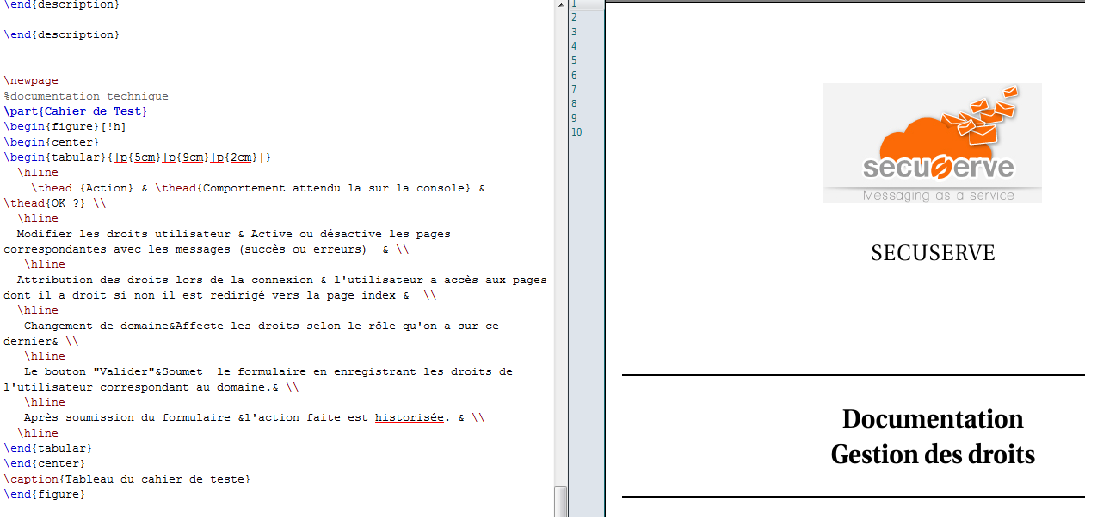
\includegraphics[width=15cm]{image/code_doc_tex.png}
\end{center}
%légende de l'image
\caption{Documentation écrite en Latex}
\end{figure}


\begin{figure}[!h]
\begin{center}
%taille de l'image en largeur
%remplacer "width" par "height" pour régler la hauteur
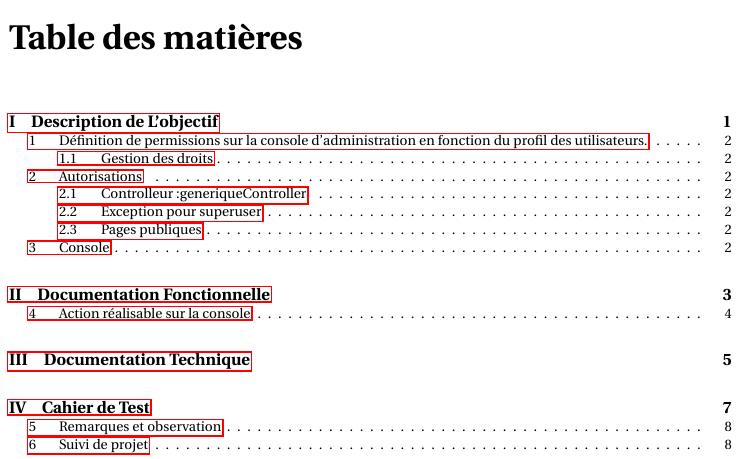
\includegraphics[width=15cm]{image/doc_somma.png}
\end{center}
%légende de l'image
\caption{Documentation écrite en Latex sommaire}
\end{figure}